\documentclass[conference]{IEEEtran}

\usepackage{amsmath,amssymb,amsfonts}
% \usepackage{algorithmic}
\usepackage{graphicx}
\usepackage[style=ieee]{biblatex}
% \usepackage{textcomp}
\usepackage{xcolor}
% \usepackage{placeins}

\addbibresource{..\\sources.bib}

\graphicspath{{.\\figures}}

\newcommand*{\norm}[1]{\left|\left|#1\right|\right|}
\newcommand{\TODO}[1]{{\LARGE \textbf{TODO}: #1}}
\newcommand*{\x}[1][i]{x^{(#1)}_t}
\newcommand*{\xdot}[1][i]{\dot{x}^{(#1)}_{t}}
\newcommand*{\xdotdot}[1][i]{\ddot{x}^{(#1)}_t}

\newcommand*{\state}[1][i]{\mathbf{x}^{(#1)}_t}
\newcommand*{\R}[1]{\mathbf{R}^{#1}}
\newcommand*{\A}{\mathbf{A}}
\newcommand*{\C}{\mathbf{C}}
\newcommand*{\W}[1][t]{\mathbf{W_{#1}}}
\newcommand*{\V}[1][t]{\mathbf{V_{#1}}}
\newcommand*{\Q}[1][t]{\mathbf{Q_{#1}}}
\newcommand*{\thet}[1][i]{\theta^{(i)}_t}

\newcommand*{\totstate}[1][t]{\mathbf{x}_{#1}}
\newcommand*{\totu}[1][t]{\mathbf{u}_{#1}}
\newcommand*{\totmeas}[1][t]{\mathbf{y}_{#1}}
\newcommand*{\f}{\mathbf{f}}
\newcommand*{\g}{\mathbf{g}}


\begin{document}

\title{Range-Based Localization Using Hybrid Optimization}

\author{\IEEEauthorblockN{Erik Helmer}
\IEEEauthorblockA{\textit{Department of Electrical Engineering} \\
\textit{Stanford University}\\
Palo Alto, USA \\
erik.helmer@stanford.edu}
}

\maketitle

\begin{abstract}
This project intends to investigate methods for solving the classic problem of range-based localization. It uses novel robust algorithms to find an optimal starting point, then uses faster methods for non-convex optimization in later time steps given the good initial guess. The goal is to estimate the paths of a group of robots over time. 

\end{abstract}

\begin{IEEEkeywords}
wireless sensor networks, localization, optimization, estimation
\end{IEEEkeywords}

\section{Introduction}
\label{sec:intro}
In a variety of applications, it is necessary to localize a group of sensors or robots. In open-air environments, this can be done with GPS. In enclosed where GPS signal is not available, it is possible to do this using a variety of SLAM techniques such as bundle adjustment or pose graph optimization (PGO). These can and have been extended to optimize over a group of robots, simultaneously determining their positions~\cite{SLAM_distributed}. However, these are dependent on a complex signal processing pipeline to extract landmark or odometry measurements to optimize over. This project intends to investigate a different approach. 

The subject of this project is an implementation and extension of a novel optimization technique for distance-based localization. This problem is described in figure~\ref{fig:problem_desc}.
\begin{figure}[ht]
    \centering
    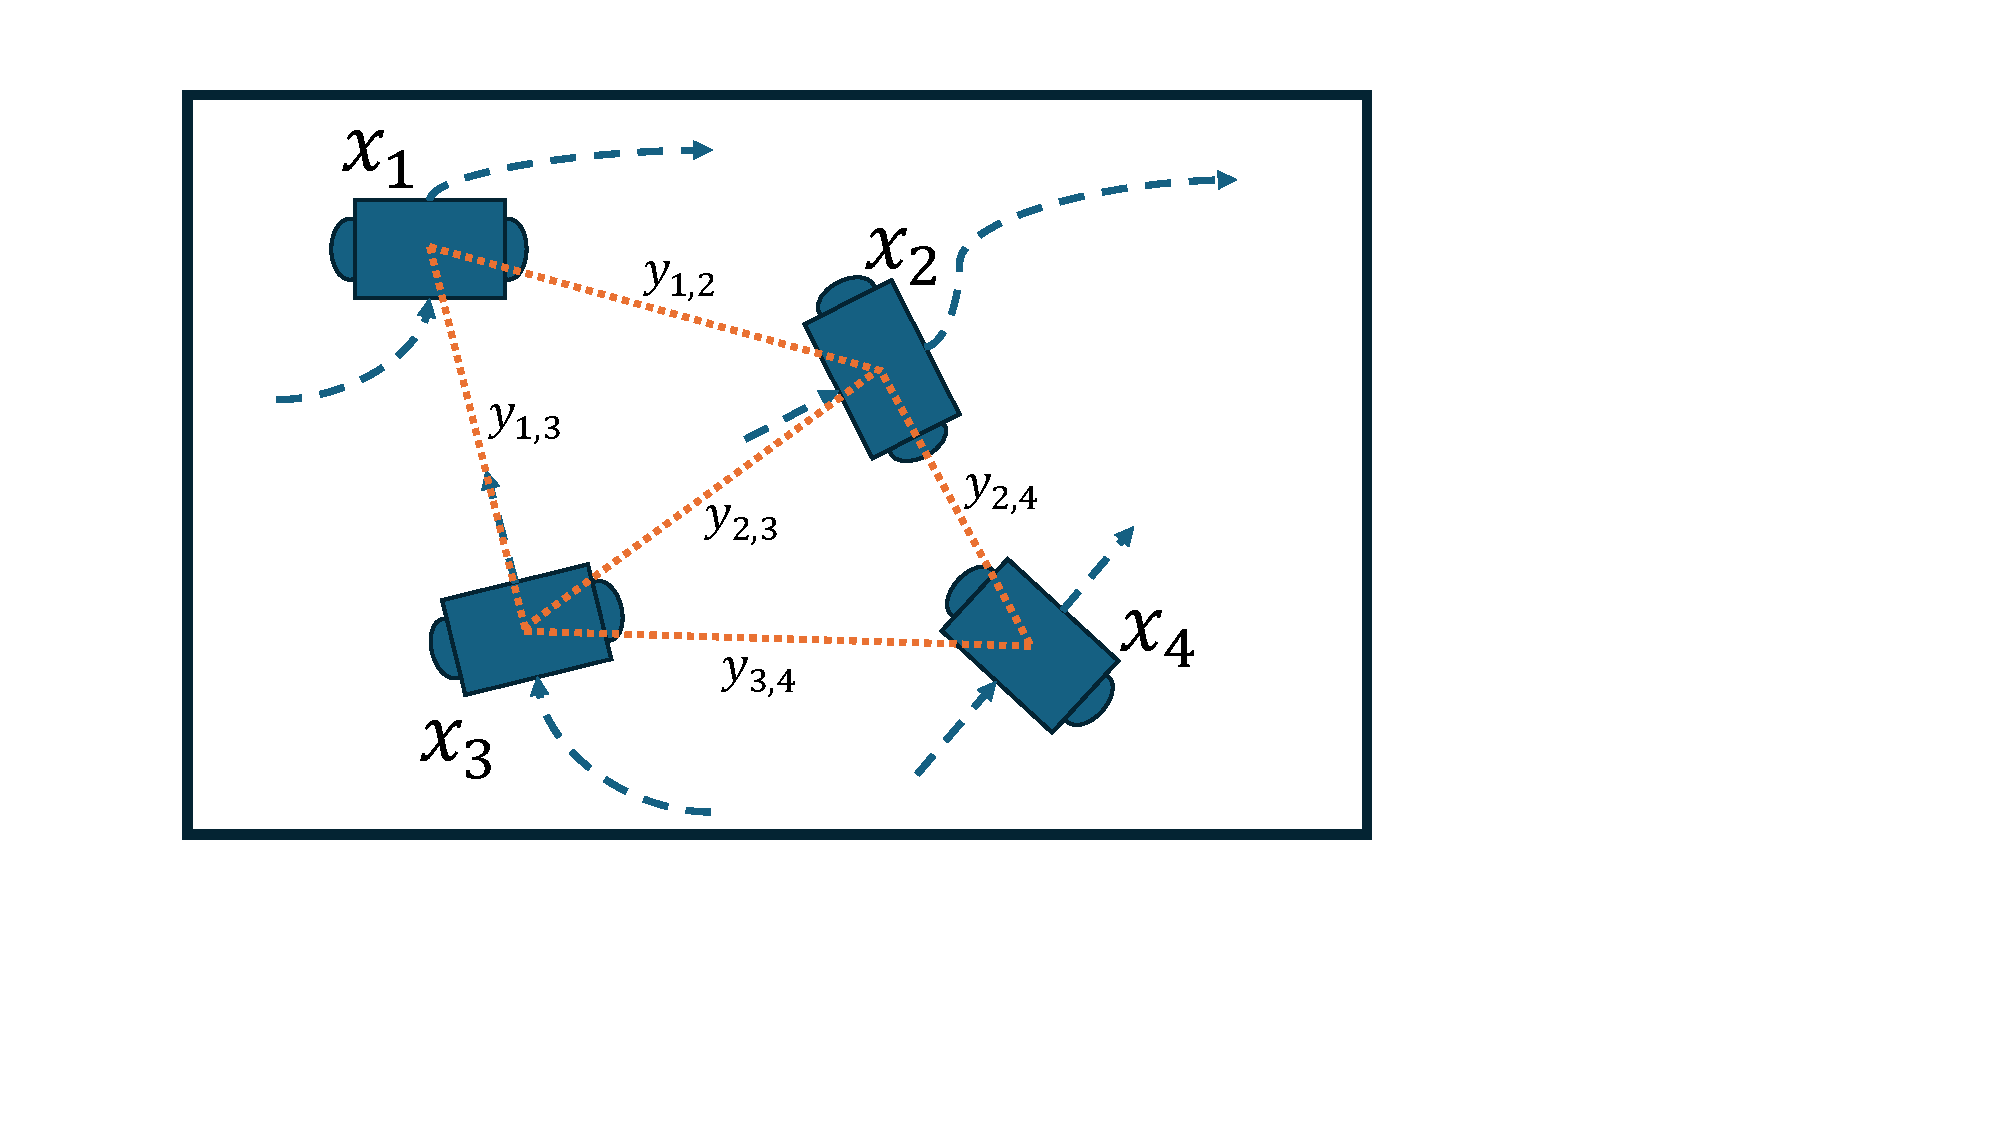
\includegraphics[width=\linewidth,trim=31mm 48mm 106mm 15mm, clip]{problem.pdf}
    \caption{Basic problem setup. In the figure, we have $N=4$ robots where $\bar{x}_i\in \mathbf{R}^n$ are the poses of the robots and $y_{i,j} \in \mathbf{R}$ are the distance measurements between them. }
    \label{fig:problem_desc}
\end{figure}
SLAM usually relies on measurements of external fixed points in the scene to extract measurements. This method would instead rely on the robots measuring only distance to each other. 

Some assumptions are made of the problem. It is assumed that while the distance measurements may be noisy, they are measurements of another robot in the group and not a false measurement of the environment. We will further assume additive Gaussian noise on the measurements. This project will not investigate the distributed case, and will instead assume centralized knowledge of all robot measurements. 

\section{Literary Review}
\label{sec:lit-rev}
The problem formulated in section~\ref{sec:intro} is usually in the literature reformulated as a graph problem, see figure~\ref{fig:problem-graph}. The measurements are interpreted as the edge weights and the positions are interpreted as vertex positions. 
% \begin{figure}[ht]
%     \centering
%     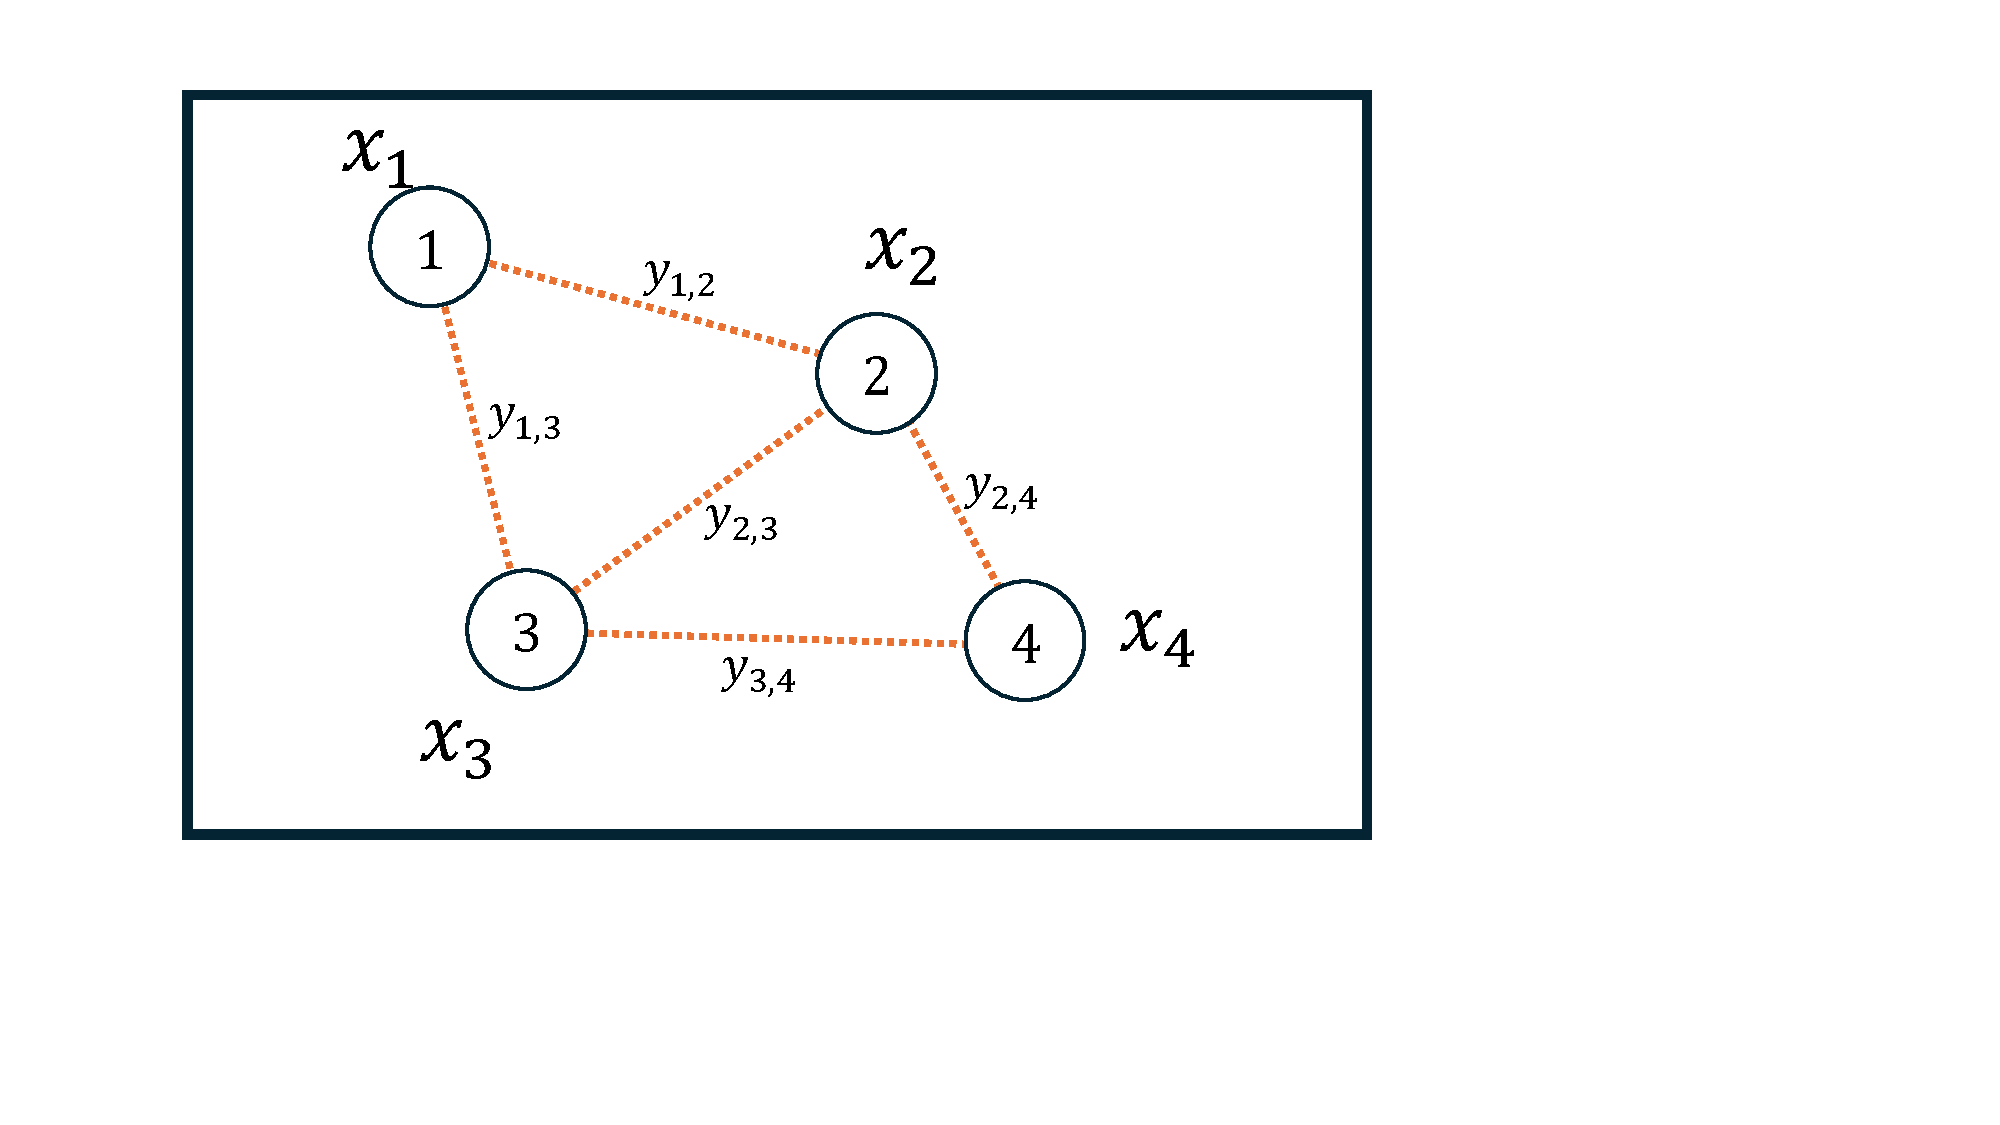
\includegraphics[width=\linewidth,trim=31mm 48mm 106mm 15mm, clip]{graph.pdf}
%     \caption{Problem reformulation. In the figure, we have a graph $\mathcal{G}=(\mathcal{V}, \mathcal{E})$ where the edges $(i, j) \in \mathcal{E}$ have weights $y_{i,j}$ and the vertices $k \in \mathcal{V}$ have positions $\bar{x}_k$.}
%     \label{fig:problem-graph}
% \end{figure}

In practice, it is rarely the case that the correspondences between robots are known without sophisticated identification algorithms using computer vision or other computationally complex methods. This is known as the anonymous localization problem, and it has been investigated by Franchi, Oriolo and Stegagno~\cite{anonymous_loc_1,anonymous_loc_2,anonymous_loc_3}. They developed a few algorithms to account for the missing correspondences by using statistical methods to simultaneously estimate multiple possible relative poses to determine the most likely correspondences. However, this markedly increases the complexity of the problem and will not be the focus of this project.

It will henceforth generally be assumed that while the measurements $y_{i,j}$ are not complete, i.e. all robots do not have measurements of every other robot, the correspondences are known. That is to say, for all measurements $y$, it is known which distance between two robots this is a measurement of. 

This problem is not new. One early approach to solve it was presented by Kruskal in \cite{Kruskal1964}. He proposed a measurement of good fit, or loss, named the stress function: 
\begin{align}
    \label{eq:kruskal-stress}
    S(x_1, ..., x_N) = \sum_{i,j} \left(
        \norm{x_i - x_j}_2 - y_{i, j}
    \right)^2
\end{align}
More accurately, Kruskal proposed a normalized version of equation~\ref{eq:kruskal-stress}, but for the purposes of this project the unnormalized version is sufficient. This function is non-convex, so iterative optimization algorithms such as gradient descent or ADMM generally converge to local minima, which necessitates a good initial guess. This algorithm will hereafter be called stress minimization in this paper.

In a companion paper, Kruskal provided a description of how to solve this problem using gradient descent~\cite{kruskal1964implementation}. Of interest to this project is the gradient that Kruskal determined. It should be noted that the stress function is non-differentiable and non-convex, so while Kruskal calls it a gradient, it is not necessarily so. Nonetheless, the stress minimization algorithm presented by Kruskal show empirically good results, so this this paper will continue with the slight abuse of notation. In addition to how do calculate the gradient of the stress function, the paper also presents a way to determine the step sizes in gradient descent. For a complete description of the algorithm, see~\cite{kruskal1964implementation}.

An alternative algorithm was proposed in~\cite{MDS_proposal} by De Leeuw. THe algorithm is called Scaling by MAjorizing a COmplicated Function (SMACOF), and it iteratively minimizes an upper bound of the stress function. Further investigated by De Leeuw in~\cite{SMACOF_convergence}, it has been proven to converge to a local minima of the stress function. However, this also requires a good initial guess to converge to a good optimum. 

These methods, while prone to local minima, can still be useful due to their simplicity when given a sufficiently good initial guess. 

In the field of sensor network localization, meaning many agents are deployed in an environment without knowledge of their positions, this problem has also been investigated. The main distinction with the robot localization problem is that authors generally assume that at least some positions known as anchors are known~\cite{WSN_collaborative,WSN_localization_techniques,optimization_WSN,WSN_stochastic}. 

Authors in these fields present additional methods of solving this problem, with different advantages and drawbacks. One technique is Particle Swarm Optimization (PSO), where a collection of particles explore the n-dimensional space to find optima~\cite{WSN_particles}. Building on this, Zhou and Chen gave a stochastic approach in~\cite{WSN_stochastic}, which finds the global optimum with high probability. 

Recently, there has been some advancements in solving the distance-based localization problem. An algorithm developed by Halsted and Schwager dubbed the Riemannian Elevator has been proposed which has better guarantees than either stress minimization or SMACOF. The complete algorithm is outside the scope of this paper, but in essence, instead of optimizing over the positions directly, it instead optimizes over an expanded $r$-dimensional Riemannian manifold of unit vectors for $r >= 2$. The solution is then projected into $2$ dimensions. It also provides a non-trivial lower bound on the provided solution. For a more thorough description, see~\cite{R_elevator}. 

\section{Proposed Work}
This project will combine some earlier approaches described in section~\ref{sec:lit-rev} to investigate whether this can improve estimation performance. The problem to be investigated, as well as the notation to be used, is described below.

\subsection{State-Space Model}
As described in section~\ref{sec:intro}, this projects seeks to investigate the problem of $n$ robots moving around in an unknown open space. The dynamics of the robots will be assumed to be \nth{1} order differential drive robot, which are robots controlled by speed $v$ and angular velocity $\omega$. This means that for each robot $i$ at time step $t$ we have 
\begin{align}
    \state = \begin{bmatrix}
        \x \\ \theta
    \end{bmatrix}
    \in \R{3} \quad \text{with} \quad \x \in \R{2}, \thet \in \R{}
\end{align}
which gives the total state
\begin{align}
    \state = \begin{bmatrix}
        \state[1] \\ \vdots \\ \state[n] 
    \end{bmatrix}
    \in \R{3n}
\end{align}

To estimate the state $\totstate$ over time we will use a extended Kalman filter (EKF). However, it will not use the distances between the robots as measurement variable. Instead, it will use the estimated positions that the optimizer algorithms determine. All robots operate independently, but we will use a single filter to estimate all of their states. With this said, update equations for a single robot $i$ are defined, below where the index $(i)$ is dropped for readability:
\begin{align}
    \totstate[t+1] &= \f(\totstate, \totu) + \W \\
    \totmeas[t+1] &= \g(\totstate) + \V
\end{align}
where
\begin{align}
    % \f(\totstate, \totu) &= \begin{bmatrix}
    %     f(\state[1], \totu^{(1)}) \\ \vdots \\ f(\state[n], \totu^{(n)})
    % \end{bmatrix} \\
    f(\totstate, \totu) &= \totstate +\Delta t
    \begin{bmatrix} 
        v \cos \theta_t \\ v \sin \theta_t \\ \omega_t
    \end{bmatrix}\\
    % \g(\totstate) &= \begin{bmatrix}
    %     g(\state[1]) \\ \vdots \\ g(\state[n])
    % \end{bmatrix} \\
    g(\totstate) &= \begin{bmatrix}
        1 & 0 & 0 \\
        0 & 1 & 0
    \end{bmatrix} \totstate \\
    \W &\sim \text{GWN} (0, \Q) \\
    \V &\sim \text{GWN} (0, \R) 
\end{align}
and where $\W$ is uncorrelated with $\V$, as well as both being uncorrelated with noise in different robots. By linearizing $f$, we get the Jacobian matrices needed by the EKF:
\begin{align}
    \mathbf{F}_t &=\begin{bmatrix}
        1 & 0 & -\Delta t v_{t} \sin(\hat{\theta}_{t \mid t}) \\
        0 & 1 & \Delta t v_{t} \cos(\hat{\theta}_{t \mid t}) \\
        0 & 0 & 1
    \end{bmatrix} \\
    \mathbf{H}_t &= \begin{bmatrix}
        1 & 0 & 0 \\
        0 & 1 & 0
    \end{bmatrix}
\end{align}
where $\hat{\theta}_{t \mid t}$ is the Kalman estimate of $\theta_t$ given measurements $\totmeas$.

\subsection{Graph Optimization} \label{sec:graphs}
% $\exists (i, j) \notin \mathcal{E}$
The positions of the robots as well as the distance measurements are modeled as a directed graph $\mathcal{G} = (\mathcal{V}, \mathcal{E})$, with $n$ vertices $i \in \mathcal{V}$ and $m$ edges $(i, j) \in \mathcal{E}$. An example configuration is shown in figure~\ref{fig:problem-graph}.
\begin{figure}[ht]
    \centering
    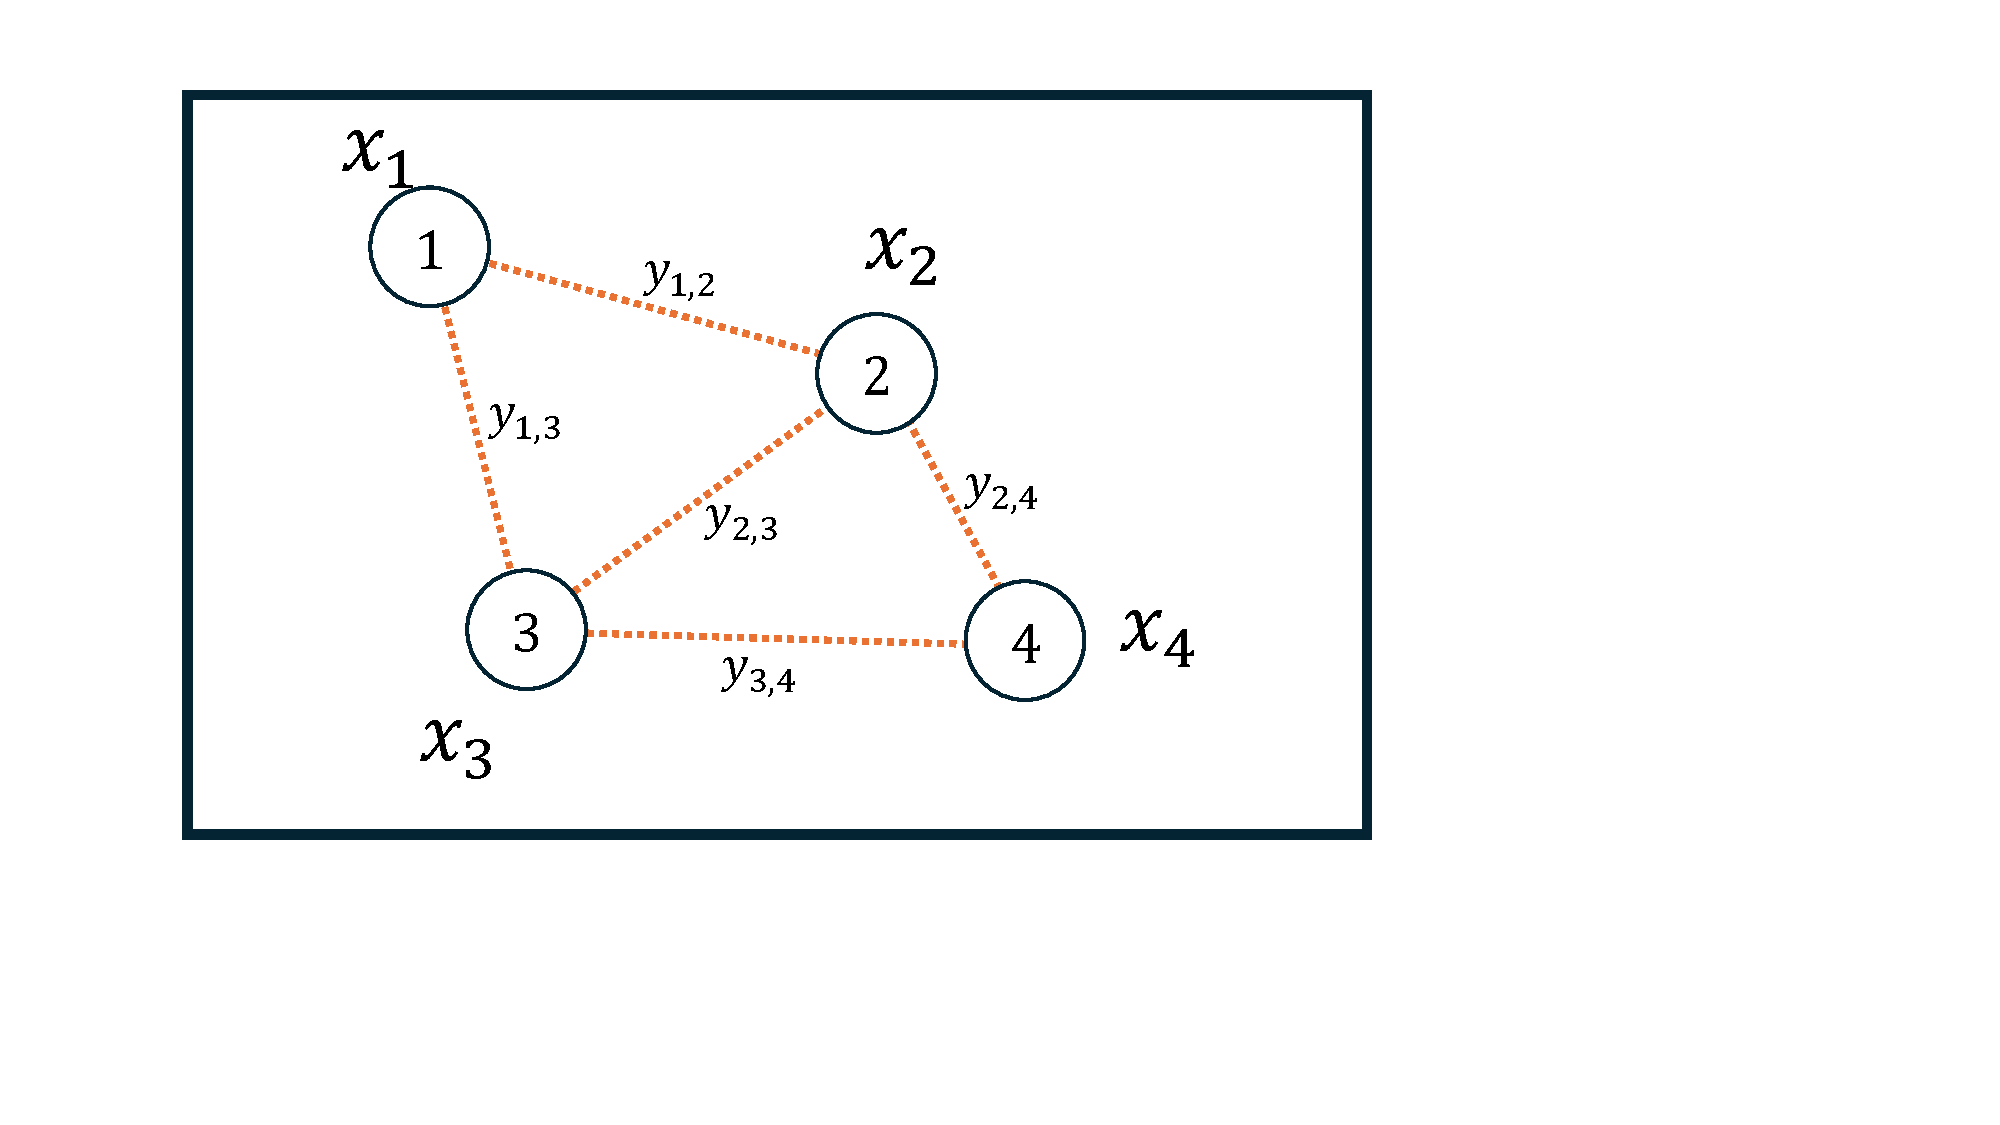
\includegraphics[width=\linewidth,trim=31mm 48mm 106mm 15mm, clip]{graph.pdf}
    \caption{Problem reformulation. In the figure, we have a graph $\mathcal{G}=(\mathcal{V}, \mathcal{E})$ where the directed edges $(i, j) \in \mathcal{E}$ have weights $l_{i,j}$ and the vertices $k \in \mathcal{V}$ have positions $x^{(k)}_t$.}
    \label{fig:problem-graph} 
\end{figure}
As described in section~\ref{sec:lit-rev}, this is a non-convex with no known efficient global solver. However, the Riemannian Elevator~\cite{R_elevator} provides an approximate solution as well as a non-trivial lower bound on the problem which we can use to determine the quality of the solution. Given this, we can approximately solve the localization problem for the initial positions. The estimates can be further refined using gradient descent on the stress minimization problem as described in previous sections. 

We use the notation defined in table~\ref{tab:notation} below to describe the graph and the data collected from it.
\FloatBarrier
\begin{table}[ht]
    \centering
    \caption{Additional definitions}
    \label{tab:notation}
    \begin{tabularx}{\linewidth}{lX}
        $\mathbf{J}_t \in \R{m \times 2}$ & 
        \textit{Connectivity matrix}.  Each row $(i, j)\in\mathcal{E}$ represents a directed edge of the graph. \\
        $\mathbf{y}_t \in \R{m}$ & 
        \textit{Measurement vector}. Each row $k$ is the distance measurement between the two nodes at row $k$ in $\mathbf{J}_t$. \\
        $\bm{\psi}_t \in \R{m}$ &
        \textit{Noise variance vector}. Each row $k$ is the variance of the noise measurement at row $k$ in $\mathbf{y}_t$. 
    \end{tabularx}
\end{table}

\subsection{Coordinate System}
Any solution to the stress minimization problem, either local or global is not unique. Since the stress function is invariant under translation, rotation, and mirroring, there is no way to determine a coordinate system matching some world coordinates. Therefore, any chosen coordinate system is as valid as any other. Initially, the Riemannian elevator is used to get estimates of the positions of the robots. This initial guess gives us the coordinate system to use in future time steps. However, when tracking the positions over longer a longer time horizon, it probable that the coordinate system will begin to drift. This means that, even though a point may have the same coordinates at two different time steps, $x^{(i)}_t = x^{(i)}_\tau$ for $t \neq \tau$, the real robot might not be at the same position at those two time steps. This is a fundamental limitation of the problem setup, as there is no measurements of the outside world. To remedy this, outside anchors could be provided which would both give a reference coordinate frame, as well as enable other localization algorithms like traditional SLAM. 

Ultimately, these are issues innate to the chosen problem, and even if the relative localization problem was solved globally, they would still persist. As such, we make no effort to solve these as the relative localization problem remains interesting regardless of limitations.

% \subsection{Unbiased Coordinates}
% Solving the localization problem, be it through the Riemannian Elevator or through stress minimization, is not enough. Since the stress function is invariant under translation, rotation, and mirroring, we need some canonical way of representing coordinates. For this, we use the mean and the SVD of the point list.

% Given a minimum of the stress function at a time $t$
% \begin{align}
%     \mathbf{X}_t = \begin{bmatrix}
%         (\x[1])^\top \\ \vdots \\ (\x[n])^\top
%     \end{bmatrix}
% \end{align}
% we subtract the mean from each point to get the same set of points centered at the origin.
% \begin{align}
%     \tilde{\mathbf{X}}_t = \begin{bmatrix}
%         (\x[1])^\top - \mu_{x_t}^\top \\ \vdots \\ (\x[n])^\top - \mu_{x_t}^\top
%     \end{bmatrix}
% \end{align}
% To cancel out rotation we determine the SVD and get 
% \begin{align}
%     U_t &\in \R{m \times 2} \\
%     \Sigma_t &\in \R{2 \times 2} \\
%     V_t &\in \R{2 \times 2}
% \end{align}
% Assuming that the two singular values are distinct, this is unique up to scaling by $\pm 1$ on the columns of $U_t$ and $V_t$. If we interpret $V_t$ as a basis for the 

% This means that the matrix 
% \begin{align}
%     U_t \Sigma_t V_t^\top V_t = U_t \Sigma_t
% \end{align}

\subsection{Algorithm Description}
With the content in previous sections, we can now define algorithm~\ref{algo:estimation}, the online estimation algorithm. For conciseness, we define the function $\text{RE}(C, \tilde{D}, W)$ the output of the Riemannian elevator, and $\text{KA}(\hat{\mathbf{x}}_{t \mid t-1}, \mathbf{y}_t, \bm{\psi}_t)$ as the output of gradient descent using Kruskal's algorithm. 



\begin{algorithm}
    \caption{Online estimation}\label{algo:estimation}
    \textbf{Inputs:} Connectivity matrix $\mathbf{J}_0$, measurement vector $\mathbf{y}_0$, noise power vector $\bm{\psi}_0$
    
    \textbf{Initialize:} Get an initial guess
    \begingroup\setstretch{1.2} % Increase line spacing
    \begin{algorithmic}[1]
        \Statex \underline{Find initial guess with Riemannian elevator}
        \State Construct matrices $C$, $\tilde{D}$, and $W$, see \cite{R_elevator}
        \State $\hat{\mathbf{X}}_0 \ \leftarrow\ \text{RE}(C, \tilde{D}, W)$
        \State Recover $\hat{\mathbf{x}}_{0 \mid 0} \in \R{3n}$ from $\hat{\mathbf{X}}_0 \in \R{n \times 2}$, assuming $\hat{\theta}^{(i)} = 0$ with high uncertainty.
    \end{algorithmic}

    \textbf{Track:} Continuously track the states
    \begin{algorithmic}[1]
        \Statex \underline{Predict}
        \State $\hat{\mathbf{x}}_{t \mid t-1} = \mathbf{f}(\hat{\mathbf{x}}_{t-1 \mid t-1}, \mathbf{u}_{t-1})$
        \State $\mathbf{P}_{t \mid t-1} = \mathbf{F}_t \mathbf{P}_{t-1 \mid t-1} \mathbf{F}_t^\top + \mathbf{Q}_t$
        \Statex \underline{Measure}
        \State Collect distance measurements $\mathbf{y}_t$
        \State Get position measurements $\mathbf{z}_t = \text{KA}(\hat{\mathbf{x}}_{t \mid t-1}, \mathbf{y}_t, \bm{\psi}_t)$ and corresponding matrices and vectors $\mathbf{J}_t$, $\mathbf{L}_t$, $\bm{\psi}_t$
        \Statex \underline{Update}
        \State $\mathbf{K}_t = \mathbf{P}_{t \mid t-1} \mathbf{H}^\top_t (\mathbf{H}_t \mathbf{P}_{t \mid t-1} \mathbf{H}_t^\top + \mathbf{R}_t)^{-1}$
        \State $\hat{\mathbf{x}}_{t \mid t} = \hat{\mathbf{x}}_{t\mid t-1} + \mathbf{K}_t (\mathbf{z}_t - \mathbf{g}(\hat{\mathbf{x}}_{t \mid t-1}))$
        \State $\mathbf{P}_{t \mid t} = (\mathbf{I} - \mathbf{K}_t \mathbf{H}_t) \mathbf{P}_{t \mid t-1}$
        \Statex \underline{Repeat}: Go to \underline{Predict}
    \end{algorithmic}
    \endgroup
\end{algorithm}

% Please number citations consecutively within brackets \cite{b1}. The 
% sentence punctuation follows the bracket \cite{b2}. Refer simply to the reference 
% number, as in \cite{b3}---do not use ``Ref. \cite{b3}'' or ``reference \cite{b3}'' except at 
% the beginning of a sentence: ``Reference \cite{b3} was the first $\ldots$''

% Number footnotes separately in superscripts. Place the actual footnote at 
% the bottom of the column in which it was cited. Do not put footnotes in the 
% abstract or reference list. Use letters for table footnotes.

% Unless there are six authors or more give all authors' names; do not use 
% ``et al.''. Papers that have not been published, even if they have been 
% submitted for publication, should be cited as ``unpublished'' \cite{b4}. Papers 
% that have been accepted for publication should be cited as ``in press'' \cite{b5}. 
% Capitalize only the first word in a paper title, except for proper nouns and 
% element symbols.

% For papers published in translation journals, please give the English 
% citation first, followed by the original foreign-language citation \cite{b6}.

\printbibliography

\end{document}
